\chapter{Electromagnetic Spectrum}
\label{ch:emspectrum}

\begin{nontechnical}
\textbf{The electromagnetic spectrum is like a piano keyboard}---but instead of sound notes, it's frequencies of light and radio waves.

\textbf{The big picture:}
\begin{itemize}
\item \textbf{Low notes (low frequency):} Radio, AM/FM, WiFi, microwaves
\item \textbf{Middle notes:} Infrared (heat from a fire), visible light (colors we see)
\item \textbf{High notes (high frequency):} Ultraviolet, X-rays, gamma rays
\end{itemize}

\textbf{It's all the same thing!} Radio waves, WiFi, light, X-rays are all electromagnetic waves---just different frequencies.

\textbf{Real-world frequencies:}
\begin{itemize}
\item \textbf{AM radio:} $\sim$1~MHz (long waves, travel far)
\item \textbf{FM radio:} $\sim$100~MHz (shorter waves, better quality)
\item \textbf{WiFi:} 2.4~GHz or 5~GHz (very short waves, fast data)
\item \textbf{Visible light:} $\sim$500~THz (that's 500,000~GHz!)
\item \textbf{X-rays:} $\sim$10$^{18}$~Hz (penetrate body)
\end{itemize}

\textbf{Why frequency matters:}
\begin{itemize}
\item \textbf{Low frequency:} Travels far, penetrates buildings, but needs big antennas
\item \textbf{High frequency:} Fast data, small antennas, but doesn't travel as far
\end{itemize}

\textbf{Fun fact:} The rainbow you see is less than 1 octave of frequency! The EM spectrum spans 20+ octaves from radio to gamma rays.
\end{nontechnical}

\section{Overview}

The \textbf{electromagnetic (EM) spectrum} encompasses all frequencies of electromagnetic radiation, from extremely low frequency (ELF) radio waves to ultra-high energy gamma rays spanning more than 20 orders of magnitude. \textbf{All EM waves travel at the speed of light} in vacuum and obey Maxwell's equations.

\begin{keyconcept}
The electromagnetic spectrum is fundamentally unified---radio waves, visible light, and gamma rays are all the same phenomenon (EM radiation) differing only in frequency and wavelength. This unity allows us to apply common propagation principles across vastly different applications.
\end{keyconcept}

Understanding the EM spectrum is essential for RF engineering, wireless communications, optical systems, and radio astronomy. Each band has unique propagation characteristics, regulatory requirements, and application domains.

\section{Mathematical Description}

\subsection{Fundamental Relationships}

The speed of light in vacuum is a fundamental constant:
\begin{equation}
c = 299{,}792{,}458 \text{ m/s} \approx 3 \times 10^8 \text{ m/s}
\end{equation}

The relationship between frequency ($f$), wavelength ($\lambda$), and propagation velocity is:
\begin{equation}
c = \lambda f
\label{eq:wavelength}
\end{equation}
where:
\begin{itemize}
\item $c$ = speed of light (m/s)
\item $\lambda$ = wavelength (meters)
\item $f$ = frequency (Hz)
\end{itemize}

From equation~\ref{eq:wavelength}, we can derive wavelength from frequency:
\begin{equation}
\lambda = \frac{c}{f} = \frac{3 \times 10^8}{f}
\end{equation}

and frequency from wavelength:
\begin{equation}
f = \frac{c}{\lambda} = \frac{3 \times 10^8}{\lambda}
\end{equation}

\subsection{Photon Energy}

From quantum mechanics, the energy of a single photon is:
\begin{equation}
E = h f = \frac{hc}{\lambda}
\end{equation}
where:
\begin{itemize}
\item $E$ = photon energy (Joules)
\item $h = 6.626 \times 10^{-34}$ J$\cdot$s = Planck's constant
\item $f$ = frequency (Hz)
\item $\lambda$ = wavelength (m)
\end{itemize}

Converting to electron-volts (eV), a common unit in photonics:
\begin{equation}
E(\text{eV}) = \frac{hf}{e} = \frac{1.24}{\lambda(\mu\text{m})}
\end{equation}
where $e = 1.602 \times 10^{-19}$ C is the elementary charge.

\subsection{Ionization Threshold}

The boundary between ionizing and non-ionizing radiation occurs at approximately:
\begin{equation}
E_{\text{ionize}} \approx 10 \text{ eV} \quad \Rightarrow \quad f_{\text{ionize}} \approx 2.4 \text{ PHz} \quad \Rightarrow \quad \lambda_{\text{ionize}} \approx 124 \text{ nm}
\end{equation}

This corresponds to the ultraviolet region. Radiation with $E > 10$~eV can eject electrons from atoms, causing chemical bond breakage and DNA damage.

\subsection{Antenna Efficiency}

For resonant antennas, optimal electrical length is typically:
\begin{equation}
L_{\text{antenna}} = \frac{n\lambda}{4}
\end{equation}
where $n$ is an odd integer (typically $n = 1$ for a quarter-wave monopole or $n = 2$ for a half-wave dipole).

The required physical antenna size scales inversely with frequency:
\begin{equation}
L_{\text{antenna}} = \frac{nc}{4f}
\end{equation}

\begin{calloutbox}{Practical Antenna Scaling}
At 100~MHz (FM radio), a half-wave dipole is $\lambda/2 = 1.5$~m long. At 10~GHz (satellite), it shrinks to just 1.5~cm. This is why higher frequencies enable compact phased arrays and mobile devices, while low-frequency systems require large antenna structures.
\end{calloutbox}

\subsection{Free-Space Path Loss}

The Friis transmission equation for free-space propagation is:
\begin{equation}
\frac{P_r}{P_t} = G_t G_r \left(\frac{\lambda}{4\pi d}\right)^2 = G_t G_r \left(\frac{c}{4\pi f d}\right)^2
\end{equation}
where:
\begin{itemize}
\item $P_r$ = received power (W)
\item $P_t$ = transmitted power (W)
\item $G_t, G_r$ = transmit/receive antenna gains (linear)
\item $d$ = distance (m)
\item $\lambda$ = wavelength (m)
\item $f$ = frequency (Hz)
\end{itemize}

Expressed in decibels, the free-space path loss is:
\begin{equation}
\text{FSPL(dB)} = 20\log_{10}(d) + 20\log_{10}(f) - 147.55
\end{equation}
where $d$ is in meters and $f$ is in Hz.

\textbf{Key insight:} Path loss increases with frequency ($+20$~dB per decade), making higher-frequency systems more challenging for long-range communications despite their smaller antennas.

\section{Spectrum Bands \& Applications}

\subsection{Electromagnetic Spectrum Visualization}

The complete EM spectrum spans from ELF radio waves at a few Hz to gamma rays above 10$^{20}$~Hz:

\begin{center}
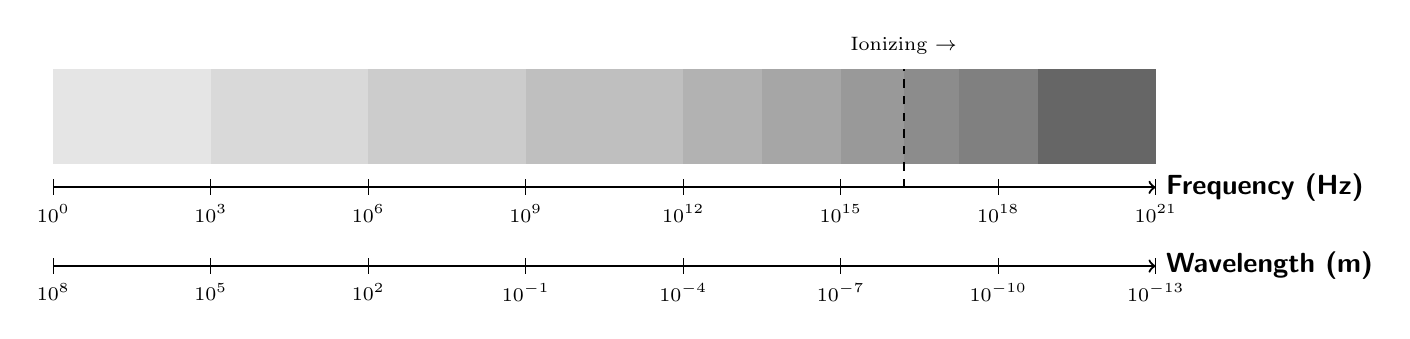
\begin{tikzpicture}[scale=1.0, font=\small]
% Frequency axis (logarithmic representation)
\draw[->,thick] (0,0) -- (14,0) node[right,font=\sffamily\bfseries] {Frequency (Hz)};

% Frequency markers (logarithmic scale)
\foreach \x/\label in {0/10$^{0}$, 2/10$^{3}$, 4/10$^{6}$, 6/10$^{9}$, 8/10$^{12}$, 10/10$^{15}$, 12/10$^{18}$, 14/10$^{21}$} {
    \draw (\x,0.1) -- (\x,-0.1) node[below,font=\scriptsize] {\label};
}

% Spectrum bands (colored boxes)
\fill[black!10] (0,0.3) rectangle (2,1.5) node[midway,align=center,font=\scriptsize\sffamily] {ELF/VLF\\Radio};
\fill[black!15] (2,0.3) rectangle (4,1.5) node[midway,align=center,font=\scriptsize\sffamily] {LF/MF/HF\\AM/SW};
\fill[black!20] (4,0.3) rectangle (6,1.5) node[midway,align=center,font=\scriptsize\sffamily] {VHF/UHF\\FM/TV/Cell};
\fill[black!25] (6,0.3) rectangle (8,1.5) node[midway,align=center,font=\scriptsize\sffamily] {SHF/EHF\\Satellite/5G};
\fill[black!30] (8,0.3) rectangle (9,1.5) node[midway,align=center,font=\scriptsize\sffamily] {THz};
\fill[black!35] (9,0.3) rectangle (10,1.5) node[midway,align=center,font=\scriptsize\sffamily] {Infrared};
\fill[black!40] (10,0.3) rectangle (10.8,1.5) node[midway,align=center,font=\scriptsize\sffamily] {Vis};
\fill[black!45] (10.8,0.3) rectangle (11.5,1.5) node[midway,align=center,font=\scriptsize\sffamily] {UV};
\fill[black!50] (11.5,0.3) rectangle (12.5,1.5) node[midway,align=center,font=\scriptsize\sffamily] {X-ray};
\fill[black!60] (12.5,0.3) rectangle (14,1.5) node[midway,align=center,font=\scriptsize\sffamily] {Gamma};

% Ionizing radiation marker
\draw[thick,dashed] (10.8,0) -- (10.8,1.5);
\node[above=2pt,font=\scriptsize] at (10.8,1.5) {Ionizing $\rightarrow$};

% Wavelength scale (bottom)
\draw[->,thick] (0,-1) -- (14,-1) node[right,font=\sffamily\bfseries] {Wavelength (m)};
\foreach \x/\label in {0/10$^{8}$, 2/10$^{5}$, 4/10$^{2}$, 6/10$^{-1}$, 8/10$^{-4}$, 10/10$^{-7}$, 12/10$^{-10}$, 14/10$^{-13}$} {
    \draw (\x,-0.9) -- (\x,-1.1) node[below,font=\scriptsize] {\label};
}

\end{tikzpicture}
\end{center}

\subsection{Radio Frequencies (RF): 3~kHz -- 300~GHz}

\subsubsection{ELF (Extremely Low Frequency): 3~Hz -- 3~kHz}

\begin{itemize}
\item \textbf{Wavelength:} 100,000~km -- 100~km
\item \textbf{Applications:} Submarine communication (penetrates seawater), geophysical surveys
\item \textbf{Propagation:} Earth-ionosphere waveguide, minimal attenuation
\item \textbf{Example:} 76~Hz US Navy submarine comms
\end{itemize}

\subsubsection{VLF (Very Low Frequency): 3~kHz -- 30~kHz}

\begin{itemize}
\item \textbf{Wavelength:} 100~km -- 10~km
\item \textbf{Applications:} Navigation (LORAN), time signals, lightning detection
\item \textbf{Propagation:} Ground wave, ionospheric reflection
\item \textbf{Example:} 24~kHz VLF navigation beacon
\end{itemize}

\subsubsection{LF (Low Frequency): 30~kHz -- 300~kHz}

\begin{itemize}
\item \textbf{Wavelength:} 10~km -- 1~km
\item \textbf{Applications:} AM radio (longwave), RFID, aviation beacons
\item \textbf{Propagation:} Ground wave (stable day/night), ionospheric at night
\item \textbf{Example:} 153~kHz longwave broadcast
\end{itemize}

\subsubsection{MF (Medium Frequency): 300~kHz -- 3~MHz}

\begin{itemize}
\item \textbf{Wavelength:} 1~km -- 100~m
\item \textbf{Applications:} AM radio (broadcast), maritime communication
\item \textbf{Propagation:} Ground wave (daytime), skywave (nighttime)
\item \textbf{Example:} 540--1600~kHz AM broadcast band
\end{itemize}

\subsubsection{HF (High Frequency): 3~MHz -- 30~MHz}

\begin{itemize}
\item \textbf{Wavelength:} 100~m -- 10~m
\item \textbf{Applications:} Shortwave radio, amateur radio, over-the-horizon radar
\item \textbf{Propagation:} Ionospheric refraction (skywave), global reach
\item \textbf{Example:} 14.2~MHz amateur band, intercontinental comms
\end{itemize}

\subsubsection{VHF (Very High Frequency): 30~MHz -- 300~MHz}

\begin{itemize}
\item \textbf{Wavelength:} 10~m -- 1~m
\item \textbf{Applications:} FM radio (88--108~MHz), TV broadcast, aviation, marine
\item \textbf{Propagation:} Line-of-sight (LOS), occasional tropospheric ducting
\item \textbf{Example:} 146~MHz amateur band, 120~MHz air traffic control
\end{itemize}

\subsubsection{UHF (Ultra High Frequency): 300~MHz -- 3~GHz}

\begin{itemize}
\item \textbf{Wavelength:} 1~m -- 10~cm
\item \textbf{Applications:} TV, cellular (GSM/LTE), GPS, WiFi (2.4~GHz), Bluetooth
\item \textbf{Propagation:} LOS, building penetration moderate, rain attenuation minimal
\item \textbf{Example:} 1.575~GHz GPS L1, 2.4~GHz ISM band
\end{itemize}

\subsubsection{SHF (Super High Frequency): 3~GHz -- 30~GHz}

\begin{itemize}
\item \textbf{Wavelength:} 10~cm -- 1~cm
\item \textbf{Applications:} Satellite comms, radar, 5G (3.5~GHz), WiFi (5--6~GHz), point-to-point links
\item \textbf{Propagation:} LOS required, rain fade significant, atmospheric absorption
\item \textbf{Example:} 5.8~GHz WiFi, 12~GHz satellite downlink (Ku-band)
\end{itemize}

\subsubsection{EHF (Extremely High Frequency): 30~GHz -- 300~GHz}

\begin{itemize}
\item \textbf{Wavelength:} 1~cm -- 1~mm
\item \textbf{Applications:} mmWave 5G (28/39~GHz), automotive radar (77~GHz), radio astronomy
\item \textbf{Propagation:} Severe rain/foliage attenuation, oxygen absorption peak at 60~GHz
\item \textbf{Example:} 39~GHz 5G, 94~GHz cloud radar
\end{itemize}

\begin{calloutbox}{60~GHz Oxygen Absorption}
At 60~GHz, atmospheric oxygen (O$_2$) has a resonant absorption peak causing $\sim$15~dB/km attenuation. This \textbf{limits range but enhances security}---signals don't travel far, preventing eavesdropping. Applications include WiGig (IEEE 802.11ad) and secure wireless backhaul links.
\end{calloutbox}

\subsection{Terahertz (THz) Gap: 300~GHz -- 10~THz}

\begin{itemize}
\item \textbf{Wavelength:} 1~mm -- 30~$\mu$m
\item \textbf{Applications:} Security imaging, spectroscopy, biomedical sensing, 6G research
\item \textbf{Propagation:} Atmospheric absorption severe (H$_2$O lines), limited range
\item \textbf{Technology:} Quantum cascade lasers (QCLs), photoconductive switches
\item \textbf{Status:} ``THz gap'' (historically difficult to generate/detect)
\end{itemize}

\textbf{Key THz features:}
\begin{itemize}
\item Non-ionizing (safe for biological tissue, unlike X-rays)
\item Penetrates clothing, paper, plastics (not metal)
\item High spatial resolution (sub-mm)
\item Strong water absorption (limits biomedical depth)
\end{itemize}

\subsection{Infrared (IR): 10~THz -- 430~THz}

\subsubsection{Far-IR (FIR): 10~THz -- 120~THz}
\begin{itemize}
\item \textbf{Wavelength:} 30~$\mu$m -- 2.5~$\mu$m
\item \textbf{Applications:} Thermal imaging, astronomy, spectroscopy
\item \textbf{Source:} Blackbody radiation (room temperature objects peak at $\sim$10~$\mu$m)
\end{itemize}

\subsubsection{Near-IR (NIR): 120~THz -- 430~THz}
\begin{itemize}
\item \textbf{Wavelength:} 2.5~$\mu$m -- 700~nm
\item \textbf{Applications:} Fiber optic comms (1550~nm), remote controls, biomedical imaging
\item \textbf{Atmospheric window:} 1.3--1.55~$\mu$m (low loss in silica fiber)
\end{itemize}

\subsection{Visible Light: 430~THz -- 750~THz}

\begin{itemize}
\item \textbf{Wavelength:} 700~nm (red) -- 400~nm (violet)
\item \textbf{Frequencies:}
  \begin{itemize}
  \item Red: $\sim$430~THz (700~nm)
  \item Yellow: $\sim$510~THz (590~nm)
  \item Green: $\sim$560~THz (535~nm)
  \item Blue: $\sim$670~THz (450~nm)
  \item Violet: $\sim$750~THz (400~nm)
  \end{itemize}
\item \textbf{Applications:} Human vision, optical comms (free-space), LiDAR, photovoltaics
\item \textbf{Energy:} 1.6--3.1~eV per photon (non-ionizing)
\end{itemize}

The solar spectrum peaks at $\sim$550~nm (green), corresponding to peak sensitivity of the human eye (photopic vision).

\subsection{Ultraviolet (UV): 750~THz -- 30~PHz}

\subsubsection{Near-UV (NUV): 750~THz -- 1.5~PHz}
\begin{itemize}
\item \textbf{Wavelength:} 400~nm -- 200~nm
\item \textbf{Applications:} Sterilization, fluorescence microscopy, photolithography
\item \textbf{Biological effects:} Tanning, vitamin D synthesis, DNA damage (UVB)
\end{itemize}

\subsubsection{Far-UV (FUV): 1.5~PHz -- 30~PHz}
\begin{itemize}
\item \textbf{Wavelength:} 200~nm -- 10~nm
\item \textbf{Applications:} Extreme sterilization, plasma diagnostics
\item \textbf{Absorption:} Strongly absorbed by atmosphere (ozone layer blocks $< 290$~nm)
\end{itemize}

\textbf{UVC ($< 280$~nm):} Germicidal (destroys DNA/RNA), used in air/water purification.

\subsection{X-Rays: 30~PHz -- 30~EHz}

\begin{itemize}
\item \textbf{Wavelength:} 10~nm -- 0.01~nm
\item \textbf{Energy:} 100~eV -- 100~keV
\item \textbf{Applications:} Medical imaging, crystallography, security screening, astronomy
\item \textbf{Generation:} Bremsstrahlung (electron deceleration), synchrotron radiation
\item \textbf{Biological effects:} \textbf{Ionizing} (breaks chemical bonds, causes mutations)
\end{itemize}

\textbf{Soft X-rays} (0.1--10~keV): Water window imaging, biological samples.

\textbf{Hard X-rays} (10--100~keV): Penetrates tissue, bone imaging (radiography).

\subsection{Gamma Rays: $>$ 30~EHz}

\begin{itemize}
\item \textbf{Wavelength:} $< 0.01$~nm
\item \textbf{Energy:} $> 100$~keV
\item \textbf{Sources:} Radioactive decay, nuclear reactions, cosmic rays, pulsars
\item \textbf{Applications:} Cancer therapy (radiotherapy), sterilization, astrophysics
\item \textbf{Detection:} Scintillation detectors, Compton scattering
\item \textbf{Biological effects:} \textbf{Highly ionizing} (severe DNA damage, cell death)
\end{itemize}

\textbf{Cosmic gamma rays:} Up to TeV energies (10$^{12}$~eV), from supernovae and black holes.

\section{Atmospheric Transmission Windows}

Earth's atmosphere is opaque to most of the EM spectrum. Only certain ``windows'' allow propagation, which determines which bands are viable for ground-based communications and astronomy.

\subsection{Atmospheric Transmission Visualization}

\begin{center}
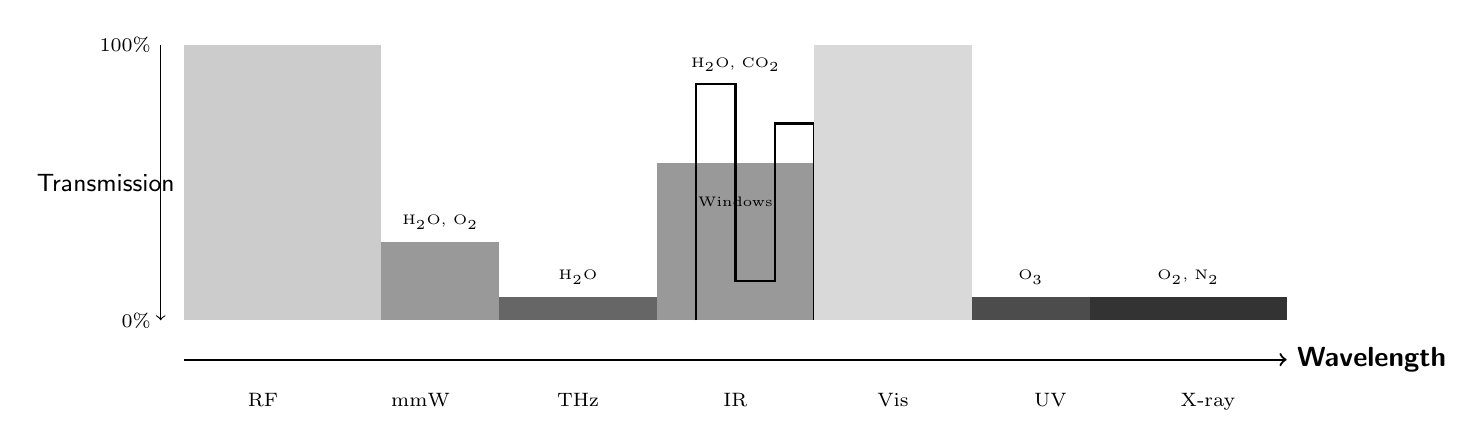
\begin{tikzpicture}[scale=1.0, font=\small]
% Frequency/wavelength axis
\draw[->,thick] (0,0) -- (14,0) node[right,font=\sffamily\bfseries] {Wavelength};

% Band labels
\foreach \x/\label in {1/RF, 3/mmW, 5/THz, 7/IR, 9/Vis, 11/UV, 13/X-ray} {
    \node[below,font=\scriptsize] at (\x,-0.3) {\label};
}

% Transmission bars (height represents transmission level)
% Radio: excellent
\fill[black!20] (0,0.5) rectangle (2.5,4) node[midway,rotate=90,font=\scriptsize] {Excellent};
% mmWave: poor
\fill[black!40] (2.5,0.5) rectangle (4,1.5) node[midway,rotate=90,font=\tiny] {Poor};
% THz: very poor
\fill[black!60] (4,0.5) rectangle (6,0.8) node[midway,font=\tiny] {Blocked};
% IR: windows
\fill[black!40] (6,0.5) rectangle (8,2.5);
\draw[thick] (6.5,0.5) -- (6.5,3.5) -- (7,3.5) -- (7,1) -- (7.5,1) -- (7.5,3) -- (8,3) -- (8,0.5);
\node[font=\tiny] at (7,2) {Windows};
% Visible: excellent
\fill[black!15] (8,0.5) rectangle (10,4) node[midway,rotate=90,font=\scriptsize] {Excellent};
% UV: blocked
\fill[black!70] (10,0.5) rectangle (11.5,0.8) node[midway,font=\tiny] {Blocked};
% X-ray/Gamma: blocked
\fill[black!80] (11.5,0.5) rectangle (14,0.8) node[midway,font=\tiny] {Blocked};

% Absorber annotations
\node[above=1pt,font=\tiny,align=center] at (3.25,1.5) {H$_2$O, O$_2$};
\node[above=1pt,font=\tiny,align=center] at (5,0.8) {H$_2$O};
\node[above=1pt,font=\tiny,align=center] at (7,3.5) {H$_2$O, CO$_2$};
\node[above=1pt,font=\tiny,align=center] at (10.75,0.8) {O$_3$};
\node[above=1pt,font=\tiny,align=center] at (12.75,0.8) {O$_2$, N$_2$};

% Axis labels
\node[left,font=\sffamily\small] at (0,2.25) {Transmission};
\draw[<-] (-0.3,0.5) -- (-0.3,4);
\node[left,font=\scriptsize] at (-0.3,0.5) {0\%};
\node[left,font=\scriptsize] at (-0.3,4) {100\%};

\end{tikzpicture}
\end{center}

\subsection{Transmission Characteristics by Band}

\begin{center}
\begin{tabular}{@{}llll@{}}
\toprule
\textbf{Band} & \textbf{Frequency/Wavelength} & \textbf{Transmission} & \textbf{Primary Absorbers} \\
\midrule
RF ($< 30$~GHz) & All RF below mmWave & Excellent & Ionosphere (HF reflection) \\
mmWave (30--300~GHz) & 1--10~mm & Poor & H$_2$O vapor, O$_2$ (60~GHz) \\
THz (0.3--10~THz) & 30~$\mu$m -- 1~mm & Very poor & H$_2$O vapor, CO$_2$ \\
Far-IR & 15--300~$\mu$m & Poor & H$_2$O, CO$_2$, O$_3$ \\
Near-IR & 0.7--2.5~$\mu$m & Good & H$_2$O (weak bands) \\
Visible & 400--700~nm & Excellent & Rayleigh scattering \\
Near-UV & 300--400~nm & Moderate & Ozone ($< 320$~nm) \\
UVC/X-ray/Gamma & $< 280$~nm & Blocked & Ozone, O$_2$, N$_2$ \\
\bottomrule
\end{tabular}
\end{center}

\textbf{Practical implications:}
\begin{itemize}
\item \textbf{Ground-to-satellite comms:} Use RF (microwaves) or optical (laser comms)
\item \textbf{THz security imaging:} Indoor only (outdoor = severe H$_2$O absorption)
\item \textbf{Radio astronomy:} ``Radio window'' (few MHz -- 30~GHz) and ``optical window'' (visible/NIR)
\end{itemize}

\section{Ionizing vs Non-Ionizing Radiation}

A critical safety and engineering distinction in the EM spectrum is the ionization threshold.

\subsection{Non-Ionizing Radiation ($< 10$~eV, $< 2.4$~PHz)}

Photon energy is insufficient to ionize atoms or break chemical bonds:

\begin{itemize}
\item \textbf{Bands:} RF, Microwave, IR, Visible, low-energy UV
\item \textbf{Effects:} Heating (dielectric loss), molecular vibration/rotation
\item \textbf{Biological effects:} Thermal (tissue heating), potential non-thermal effects (debated)
\item \textbf{Safety metric:} Specific Absorption Rate (SAR, W/kg)
\end{itemize}

\textbf{Example:} WiFi at 2.4~GHz has photon energy:
\begin{equation}
E = hf = (6.626 \times 10^{-34})(2.4 \times 10^9) = 1.59 \times 10^{-24} \text{ J} = 10^{-5} \text{ eV}
\end{equation}

This is \textbf{6 orders of magnitude below} the ionization threshold---effects are purely thermal.

\subsection{Ionizing Radiation ($> 10$~eV, $> 2.4$~PHz)}

Photon energy is sufficient to eject electrons from atoms:

\begin{itemize}
\item \textbf{Bands:} High-energy UV, X-rays, Gamma rays
\item \textbf{Effects:} Breaks chemical bonds, damages DNA, creates free radicals
\item \textbf{Biological effects:} Mutations, cancer, acute radiation syndrome (high dose)
\item \textbf{Safety metric:} Absorbed dose (Gray, Gy) and effective dose (Sievert, Sv)
\end{itemize}

The ionization threshold for biological molecules is approximately:
\begin{equation}
E_{\text{threshold}} \approx 10 \text{ eV} \quad \text{(single ionization)}
\end{equation}

Double-strand DNA breaks (irreversible damage) occur at approximately:
\begin{equation}
E_{\text{DNA break}} \approx 20 \text{ eV}
\end{equation}

\begin{warningbox}
\textbf{X-ray example:} A 30~keV X-ray photon carries 30,000~eV of energy, sufficient to cause \textbf{1,500 ionization events} or multiple DNA strand breaks. This is why X-ray exposure must be carefully controlled and justified by medical necessity.
\end{warningbox}

\section{Frequency Allocation \& Regulation}

The \textbf{International Telecommunication Union (ITU)} coordinates global spectrum allocation to prevent interference and ensure equitable access.

\subsection{Key Allocated Bands}

\begin{center}
\begin{tabular}{@{}lll@{}}
\toprule
\textbf{Service} & \textbf{Frequency} & \textbf{Regulation} \\
\midrule
AM Radio & 530--1710~kHz & Licensed broadcast \\
FM Radio & 88--108~MHz & Licensed broadcast \\
Aviation & 108--137~MHz & Protected (safety of life) \\
Marine VHF & 156--162~MHz & Regulated \\
GPS & 1.176--1.575~GHz & Protected (military/civilian) \\
WiFi (2.4~GHz) & 2.400--2.4835~GHz & \textbf{ISM band} (unlicensed) \\
WiFi (5~GHz) & 5.150--5.850~GHz & \textbf{U-NII} (unlicensed) \\
Cellular (LTE/5G) & 600--6000~MHz & Licensed (carriers) \\
5G mmWave & 24--47~GHz & Licensed (auction) \\
Satellite (Ka-band) & 26.5--40~GHz & Licensed \\
\bottomrule
\end{tabular}
\end{center}

\subsection{ISM Bands}

\textbf{Industrial, Scientific, Medical (ISM)} bands are unlicensed, allowing shared use without licensing fees:

\begin{itemize}
\item 902--928~MHz (US only)
\item 2.400--2.500~GHz (global)
\item 5.725--5.875~GHz (global)
\end{itemize}

Trade-off: Higher interference potential, no guaranteed quality of service.

\section{Wavelength vs Antenna Size}

\textbf{Rule of thumb:} Efficient antennas are typically $\lambda/2$ or $\lambda/4$ in size.

\subsection{Antenna Size Scaling}

\begin{center}
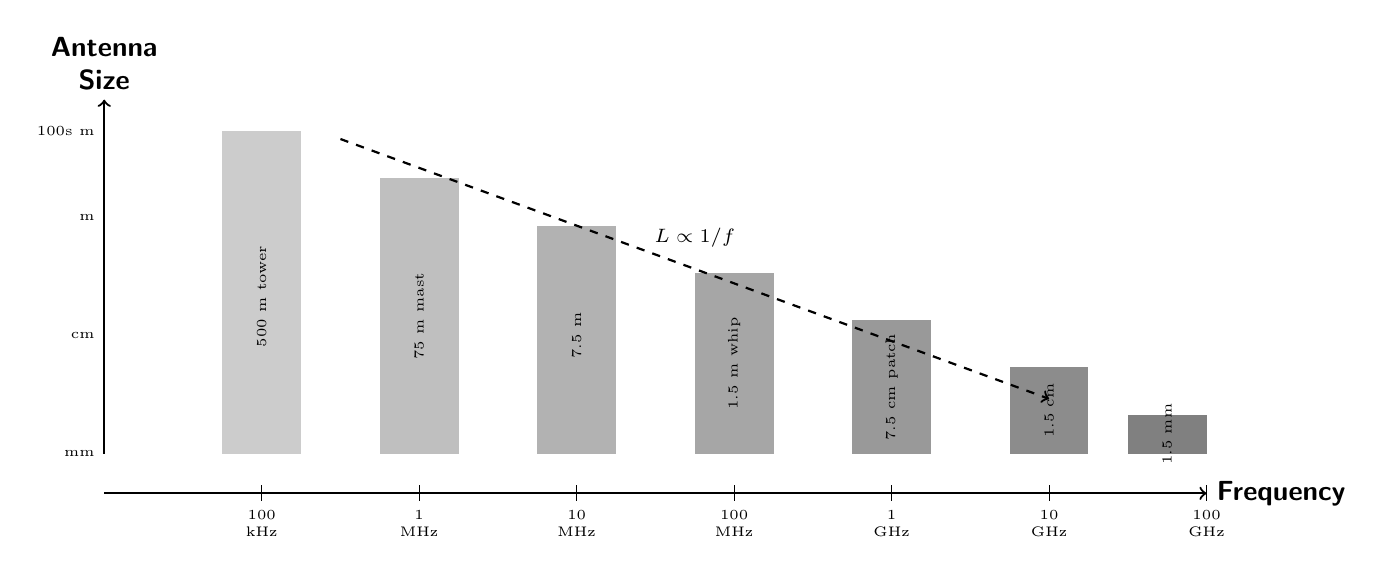
\begin{tikzpicture}[scale=1.0, font=\small]
% Logarithmic frequency axis (horizontal)
\draw[->,thick] (0,0) -- (14,0) node[right,font=\sffamily\bfseries] {Frequency};

% Frequency markers
\foreach \x/\label in {2/100\\kHz, 4/1\\MHz, 6/10\\MHz, 8/100\\MHz, 10/1\\GHz, 12/10\\GHz, 14/100\\GHz} {
    \draw (\x,0.1) -- (\x,-0.1) node[below,font=\tiny,align=center] {\label};
}

% Antenna size bars (height represents antenna length, inversely proportional to frequency)
% Using logarithmic scaling: height = 5 - 0.6*position
\fill[black!20] (1.5,0.5) rectangle (2.5,4.6);
\node[rotate=90,font=\tiny] at (2,2.5) {500 m tower};

\fill[black!25] (3.5,0.5) rectangle (4.5,4);
\node[rotate=90,font=\tiny] at (4,2.25) {75 m mast};

\fill[black!30] (5.5,0.5) rectangle (6.5,3.4);
\node[rotate=90,font=\tiny] at (6,2) {7.5 m};

\fill[black!35] (7.5,0.5) rectangle (8.5,2.8);
\node[rotate=90,font=\tiny] at (8,1.65) {1.5 m whip};

\fill[black!40] (9.5,0.5) rectangle (10.5,2.2);
\node[rotate=90,font=\tiny] at (10,1.35) {7.5 cm patch};

\fill[black!45] (11.5,0.5) rectangle (12.5,1.6);
\node[rotate=90,font=\tiny] at (12,1.05) {1.5 cm};

\fill[black!50] (13,0.5) rectangle (14,1);
\node[rotate=90,font=\tiny] at (13.5,0.75) {1.5 mm};

% Vertical axis
\draw[->,thick] (0,0.5) -- (0,5) node[above,font=\sffamily\bfseries,align=center] {Antenna\\Size};
\node[left,font=\tiny] at (0,0.5) {mm};
\node[left,font=\tiny] at (0,2) {cm};
\node[left,font=\tiny] at (0,3.5) {m};
\node[left,font=\tiny] at (0,4.6) {100s m};

% Annotation showing inverse relationship
\draw[->,dashed,thick] (3,4.5) -- (12,1.2);
\node[above,font=\scriptsize] at (7.5,3) {$L \propto 1/f$};

\end{tikzpicture}
\end{center}

\textbf{Practical antenna scaling rule:}
\begin{equation}
L_{\text{antenna}} = \frac{n\lambda}{4} = \frac{nc}{4f}
\end{equation}
where $n$ is typically 1 (quarter-wave) or 2 (half-wave).

\subsection{Antenna Size Examples}

\begin{center}
\begin{tabular}{@{}lll@{}}
\toprule
\textbf{Frequency} & \textbf{Wavelength} & \textbf{Typical Antenna} \\
\midrule
150~kHz (LF) & 2000~m & 500~m tower (impractical!) \\
1~MHz (AM) & 300~m & 75~m vertical mast \\
100~MHz (FM) & 3~m & 1.5~m whip ($\lambda/2$ dipole) \\
1~GHz (cellular) & 30~cm & 7.5~cm patch ($\lambda/4$) \\
10~GHz (satellite) & 3~cm & 1.5~cm patch array \\
300~GHz (mmWave) & 1~mm & 0.25~mm array element \\
1.875~THz & 160~$\mu$m & 40~$\mu$m aperture \\
\bottomrule
\end{tabular}
\end{center}

\textbf{Key trade-off:} Higher frequencies enable \textbf{compact antennas and phased arrays}, but suffer from increased propagation loss.

\section{Worked Example: Link Budget Across Frequency Bands}

Compare a 1~km wireless link operating at three different frequencies: 900~MHz (UHF), 5.8~GHz (SHF), and 60~GHz (EHF).

\subsection*{Given Parameters}

\begin{tabular}{@{}ll@{}}
Transmit power & $P_t = 1$~W = 30~dBm \\
Distance & $d = 1$~km = 1000~m \\
Antenna gains & $G_t = G_r = 0$~dBi (isotropic) \\
\end{tabular}

\subsection*{Required}

Calculate the received power and free-space path loss at each frequency.

\subsection*{Solution}

\textit{Step 1: Calculate free-space path loss using equation~\ref{eq:fspl}}

The FSPL in decibels is:
\begin{equation}
\text{FSPL(dB)} = 20\log_{10}(d) + 20\log_{10}(f) - 147.55
\label{eq:fspl}
\end{equation}

\textit{Step 2: Calculate for 900~MHz (UHF)}
\begin{equation}
\text{FSPL}_{900} = 20\log_{10}(1000) + 20\log_{10}(900 \times 10^6) - 147.55 = 91.5 \text{ dB}
\end{equation}

\textit{Step 3: Calculate for 5.8~GHz (SHF)}
\begin{equation}
\text{FSPL}_{5800} = 20\log_{10}(1000) + 20\log_{10}(5.8 \times 10^9) - 147.55 = 107.7 \text{ dB}
\end{equation}

\textit{Step 4: Calculate for 60~GHz (EHF)}
\begin{equation}
\text{FSPL}_{60000} = 20\log_{10}(1000) + 20\log_{10}(60 \times 10^9) - 147.55 = 128.0 \text{ dB}
\end{equation}

\textit{Step 5: Calculate received power}

With $G_t = G_r = 0$~dBi and $P_t = 30$~dBm:
\begin{equation}
P_r(\text{dBm}) = P_t(\text{dBm}) + G_t + G_r - \text{FSPL(dB)}
\end{equation}

\begin{itemize}
\item \textbf{900~MHz:} $P_r = 30 + 0 + 0 - 91.5 = -61.5$~dBm
\item \textbf{5.8~GHz:} $P_r = 30 + 0 + 0 - 107.7 = -77.7$~dBm
\item \textbf{60~GHz:} $P_r = 30 + 0 + 0 - 128.0 = -98.0$~dBm
\end{itemize}

\subsection*{Interpretation}

The 60~GHz link suffers \textbf{36.5~dB more path loss} than the 900~MHz link over the same distance. This demonstrates why:
\begin{itemize}
\item Lower frequencies (UHF) are preferred for long-range communications
\item Higher frequencies (mmWave) require higher antenna gains or shorter ranges
\item The ``free'' spectrum at mmWave comes with significant propagation challenges
\end{itemize}

To achieve comparable performance, the 60~GHz link would need \textbf{+36.5~dB additional antenna gain} (e.g., directional antennas or phased arrays).

\section{Spectrum Utilization Trends}

\subsection{Historical Progression}

\begin{itemize}
\item \textbf{1900s:} MF/HF (AM radio, maritime communications)
\item \textbf{1950s:} VHF/UHF (FM radio, TV broadcast, early mobile)
\item \textbf{1990s:} SHF (cellular 2G/3G, WiFi, GPS)
\item \textbf{2010s:} EHF (5G mmWave, 60~GHz WiGig)
\item \textbf{2020s:} THz (security imaging, 6G research, biomedical applications)
\end{itemize}

\subsection{Primary Driver: Spectrum Congestion}

As lower frequency bands become saturated, systems migrate to higher frequencies:

\begin{itemize}
\item \textbf{VHF/UHF:} Highly congested, licensed, expensive
\item \textbf{SHF/EHF (mmWave):} Abundant spectrum, GHz of bandwidth available
\item \textbf{THz:} Virtually unlimited, atmospheric absorption limits outdoor range
\end{itemize}

\textbf{Capacity relationship:}
\begin{equation}
C = B \log_2(1 + \text{SNR})
\end{equation}
where $C$ = channel capacity (bps), $B$ = bandwidth (Hz), SNR = signal-to-noise ratio.

Higher frequencies offer more bandwidth ($B$), enabling higher data rates despite propagation challenges.

\section{Propagation Characteristics by Band}

\subsection{Long Wavelengths (LF/MF/HF)}

\textbf{Advantages:}
\begin{itemize}
\item Ground wave propagation (stable, follows Earth curvature)
\item Ionospheric reflection (HF skywave $\rightarrow$ global reach)
\item Penetrates buildings, foliage, seawater
\end{itemize}

\textbf{Disadvantages:}
\begin{itemize}
\item Large antennas required (10s to 100s of meters)
\item Low bandwidth (kHz range)
\item Crowded spectrum, highly regulated
\end{itemize}

\subsection{Medium Wavelengths (VHF/UHF)}

\textbf{Advantages:}
\begin{itemize}
\item Moderate antenna size (cm to meters)
\item Good building penetration (especially lower UHF)
\item Balanced range vs bandwidth trade-off
\end{itemize}

\textbf{Disadvantages:}
\begin{itemize}
\item Line-of-sight propagation dominates
\item Spectrum congestion, competitive licensing
\end{itemize}

\subsection{Short Wavelengths (SHF/EHF/THz)}

\textbf{Advantages:}
\begin{itemize}
\item Huge bandwidth available (GHz)
\item Small antennas enable phased arrays
\item Narrow beams (spatial reuse, security)
\end{itemize}

\textbf{Disadvantages:}
\begin{itemize}
\item Severe atmospheric attenuation (rain, oxygen, water vapor)
\item Minimal building penetration
\item Requires line-of-sight

\end{itemize}

\textbf{Atmospheric attenuation rates:}
\begin{equation}
\alpha_{60\text{GHz}} \approx 15 \text{ dB/km} \quad \text{(oxygen absorption)}
\end{equation}
\begin{equation}
\alpha_{\text{THz}} > 100 \text{ dB/km} \quad \text{(water vapor)}
\end{equation}

\section{Applications}

\subsection{GPS Navigation (1.575~GHz, L-band)}

The Global Positioning System operates in the L-band for optimal propagation:
\begin{itemize}
\item \textbf{Frequency:} L1 carrier at 1.575~GHz
\item \textbf{Modulation:} BPSK with spread spectrum
\item \textbf{Advantages:} Good atmospheric penetration, moderate ionospheric delay
\item \textbf{Challenge:} Low received power ($\sim$-130~dBm), requires sensitive receivers
\item \textbf{Applications:} Navigation, timing synchronization, geodesy
\end{itemize}

\subsection{WiFi (2.4~GHz and 5~GHz, ISM bands)}

IEEE 802.11 wireless LANs exploit unlicensed ISM bands:
\begin{itemize}
\item \textbf{2.4~GHz band:} Better building penetration, more interference
\item \textbf{5~GHz band:} Higher bandwidth, less congestion, shorter range
\item \textbf{Standards:} 802.11n/ac/ax (WiFi 4/5/6)
\item \textbf{Data rates:} Up to 9.6~Gbps (WiFi 6E)
\item \textbf{Applications:} Home/office networking, IoT devices
\end{itemize}

\subsection{5G mmWave (28/39~GHz)}

Fifth-generation cellular exploits mmWave for ultra-high bandwidth:
\begin{itemize}
\item \textbf{Frequency bands:} 24--47~GHz (varies by region)
\item \textbf{Bandwidth:} 100--400~MHz per channel
\item \textbf{Peak rates:} 10+ Gbps
\item \textbf{Beamforming:} Phased arrays compensate for high path loss
\item \textbf{Range:} Typically $< 500$~m, urban environments
\item \textbf{Applications:} Fixed wireless access, enhanced mobile broadband
\end{itemize}

\subsection{Fiber Optic Communications (1550~nm, Near-IR)}

Silica optical fiber has minimum loss at 1550~nm (193~THz):
\begin{itemize}
\item \textbf{Attenuation:} 0.2~dB/km (vs 15~dB/km at 60~GHz!)
\item \textbf{Technology:} Wavelength-division multiplexing (WDM)
\item \textbf{Capacity:} 10s of Tbps per fiber
\item \textbf{Distance:} 1000s of km with optical amplifiers
\item \textbf{Applications:} Internet backbone, submarine cables, data centers
\end{itemize}

\subsection{Medical X-Ray Imaging (30~keV -- 100~keV)}

X-ray photons penetrate tissue for diagnostic imaging:
\begin{itemize}
\item \textbf{Energy:} 30--100~keV (typical diagnostic range)
\item \textbf{Wavelength:} 0.01--0.04~nm
\item \textbf{Contrast:} Bone absorbs more than soft tissue
\item \textbf{Dose:} Typical chest X-ray $\sim$0.1~mSv
\item \textbf{Applications:} Radiography, fluoroscopy, CT scans
\end{itemize}

\section{Summary}

\subsection{Spectrum at a Glance}

\begin{center}
\small
\begin{tabular}{@{}llllll@{}}
\toprule
\textbf{Band} & \textbf{Frequency} & \textbf{Wavelength} & \textbf{Key Apps} & \textbf{Propagation} & \textbf{Ionizing?} \\
\midrule
ELF & 3~Hz--3~kHz & 100,000--100~km & Submarine & Waveguide & No \\
VLF & 3--30~kHz & 100--10~km & Navigation & Ground wave & No \\
LF & 30--300~kHz & 10--1~km & RFID & Ground/iono & No \\
MF & 300~kHz--3~MHz & 1~km--100~m & AM radio & Ground/sky & No \\
HF & 3--30~MHz & 100--10~m & Shortwave & Ionospheric & No \\
VHF & 30--300~MHz & 10--1~m & FM/TV & LOS & No \\
UHF & 300~MHz--3~GHz & 1~m--10~cm & Cell/WiFi & LOS & No \\
SHF & 3--30~GHz & 10--1~cm & Satellite & Rain fade & No \\
EHF & 30--300~GHz & 1~cm--1~mm & mmWave 5G & Severe loss & No \\
THz & 0.3--10~THz & 1~mm--30~$\mu$m & Imaging & Limited & No \\
IR & 10--430~THz & 30~$\mu$m--700~nm & Thermal/fiber & Windows & No \\
Visible & 430--750~THz & 700--400~nm & Vision & Excellent & No \\
UV & 750~THz--30~PHz & 400--10~nm & Sterilization & Absorbed & Partial \\
X-ray & 30~PHz--30~EHz & 10--0.01~nm & Medical & Blocked & \textbf{Yes} \\
Gamma & $>$ 30~EHz & $<$ 0.01~nm & Therapy & Blocked & \textbf{Yes} \\
\bottomrule
\end{tabular}
\end{center}

\subsection{Key Insights}

\begin{itemize}
\item \textbf{Unified phenomenon:} All EM radiation obeys Maxwell's equations; differences arise from frequency-dependent interactions with matter
\item \textbf{Antenna scaling:} Antenna size $\propto 1/f$, enabling compact devices at high frequencies
\item \textbf{Path loss:} Free-space loss increases with frequency ($+20$~dB per decade)
\item \textbf{Atmospheric windows:} Only RF ($< 30$~GHz) and visible/NIR bands have good atmospheric transmission
\item \textbf{Ionization threshold:} $\sim$10~eV ($\sim$2.4~PHz) separates safe (non-ionizing) from hazardous (ionizing) radiation
\item \textbf{Spectrum congestion:} Drives migration to higher frequencies (mmWave, THz) despite propagation challenges
\end{itemize}

\section{Further Reading}

\textbf{Foundation concepts:}
\begin{itemize}
\item Chapter~\ref{ch:maxwell}: Maxwell's Equations and Wave Propagation---mathematical foundation of EM waves
\item Chapter~\ref{ch:fspl}: Free-Space Path Loss---frequency-dependent propagation loss calculations
\item Chapter~\ref{ch:iq}: IQ Representation---complex baseband representation used across the spectrum
\end{itemize}

\textbf{Specific frequency bands:}
\begin{itemize}
\item Chapter~\ref{ch:thz}: Terahertz Technology---applications and challenges in the THz gap
\item Chapter~\ref{ch:mmwave}: mmWave Communications---5G and beyond at 30--300~GHz
\item Chapter~\ref{ch:optical}: Optical Communications---fiber optic systems in the near-IR
\end{itemize}

\textbf{System design:}
\begin{itemize}
\item Chapter~\ref{ch:antenna}: Antenna Theory---design principles for frequency-specific antennas
\item Chapter~\ref{ch:linkbudget}: Link Budget Analysis---comprehensive system design across bands
\item Chapter~\ref{ch:propagation}: Atmospheric Propagation---absorption, refraction, and ducting effects
\end{itemize}

\textbf{Applications:}
\begin{itemize}
\item Chapter~\ref{ch:bpsk}: Binary Phase-Shift Keying---modulation used in GPS and satellite systems
\item Chapter~\ref{ch:fsk}: Frequency-Shift Keying---common in ISM band applications
\item Chapter~\ref{ch:ofdm}: OFDM---multi-carrier modulation for WiFi and LTE
\end{itemize}
